
%{\bfseries Definition 1: } {\itshape$(k-\omega)$ coverage}
%\subsubsection{($k-\omega$) region of a k-sensor list}
\begin{df} 
{\itshape$(k-\omega)$ coverage}
\begin{itemize}
	\item A point $P$ is said to be $(k-\omega)$ covered if there exists a list of $k$ sensors $L = \{S_1, S_2,...,S_k\}$ ordered in counter-clockwise order around $P$, such that $\omega < (\overrightarrow{PS_i}, \overrightarrow{PS_{i+1}}) < \pi, \forall i \in \{1,2,...,k\}$.
	\item A region $R$ is said to be $(k-\omega)$ covered if every point in $R$ is $(k-\omega)$ covered.
\end{itemize}
\end{df}
\begin{df}
{\itshape Inner safe region of a polygon's side.}\par
Given a polygon {\sc pol}. Let $AB$ is a side of {\sc pol}. The way to determine the inner safe region is as follows:
%\vspace{-5pt}
\begin{itemize}
	\item Choose the midpoint $M$ of $AB$.
	\item Draw an arrow from $M$ toward the inner region of {\sc pol}.
	\item The safe region of $AB$ consists 2 symmetrical parts splitted by line $AB$. The part that the arrow points to is the inner safe region of $AB$.
\end{itemize}
\end{df}
Figure ~\ref{innersafe} is an illustration of inner safe region of $S_1S_2$.
\begin{figure}[!h]
	\begin{center}
	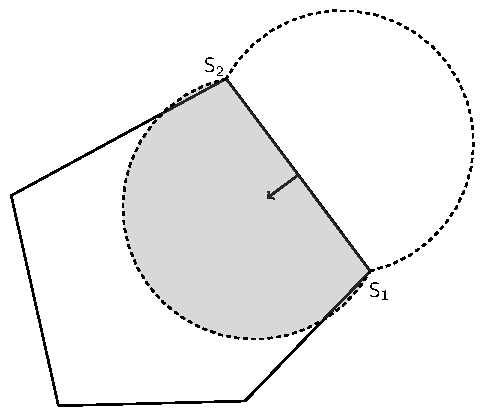
\includegraphics[scale=1.]{innersafe.pdf}	
	\caption{inner safe region of $S_1S_2$}
	\label{innersafe}
	\end{center}
\end{figure}
\begin{df}
{\itshape($k-\omega$) region of an $k$-sensor ordered list}\\
Given a $k$-sensor ordered list $L = \{S_1,S_2,...,S_k\}$. ($k-\omega$) region of $L$ is the locus of points that are ($k-\omega$) covered by $L$.
\end{df}
\begin{thr}
{\itshape($k-\omega$) region of an $k$-sensor ordered list $L =\{S_1,S_2,...,S_k\}$ is the intersection of inner safe region of every line segment $S_iS_{i+1}$ and the sensing range of all sensors in $L$}.
\end{thr}
\begin{pf}
	Let $R$ denote the ($k-\omega$) region of $L$. We only consider the case that $R$ is not empty. Suppose that $P$ is a point inside $R$, then $P$ is ($k-\omega$) covered by $L$. From definition 1, we have $(\overrightarrow{PS_i}, \overrightarrow{PS_{i+1}}) > \omega$ (1) and $(\overrightarrow{PS_i}, \overrightarrow{PS_{i+1}}) < \pi$ (2),\ $\forall i \in \{1,2,...,k\}$. Condition (1) means that $P$ is inside the safe region of $S_iS_{i+1}$. This safe region has 2 symmetrical parts splitted by line $S_iS_{i+1}$. Condition (2) forces $P$ to be located at only one special part which satisfies $(\overrightarrow{PS_i}, \overrightarrow{PS_{i+1}}) < \pi$. And this part is always the inner safe region of $S_iS_{i+1}$. Hence, $P$ is inside the intersection of inner safe region of every line segment $S_iS_{i+1},\ i=\overline{1,k}$ and the sensing region of all sensors in $L$ (call this intersection $\mho$) (*).\par
\indent On the other hand, if $P$ is inside $\mho$, $P$ satisfies the condition (1) and (2). Thus, $P$ is ($k-\omega$) covered by $L$, which deduce to $P$ is inside $R$ (**).\par
\indent From (*) and (**), we have theorem 1 proved.
\end{pf}
\begin{thr}
{\itshape($k-\omega$) region of an $k$-sensor ordered list $L =\{S_1,S_2,...,S_k\}$ is a convex region}.
\end{thr}
\begin{pf}
The intersection of two convex regions is a convex region. Hence, the intersection of any limited sets of convex region is a convex region. From theorem 1, it is obviously that ($k-\omega$) region of a list $L$ is intersections of convex regions and thus, we have theorem 2 proved.
\end{pf}
Figure 2 is an illustration of this theorem. By that, the blue hatching area is the ($k-\omega$) region of $L=\{S_1,S_2,S_3,S_4\}$ and $\omega = 60$.
\begin{figure}[h]
\begin{minipage}{.5\linewidth}
	\centering
	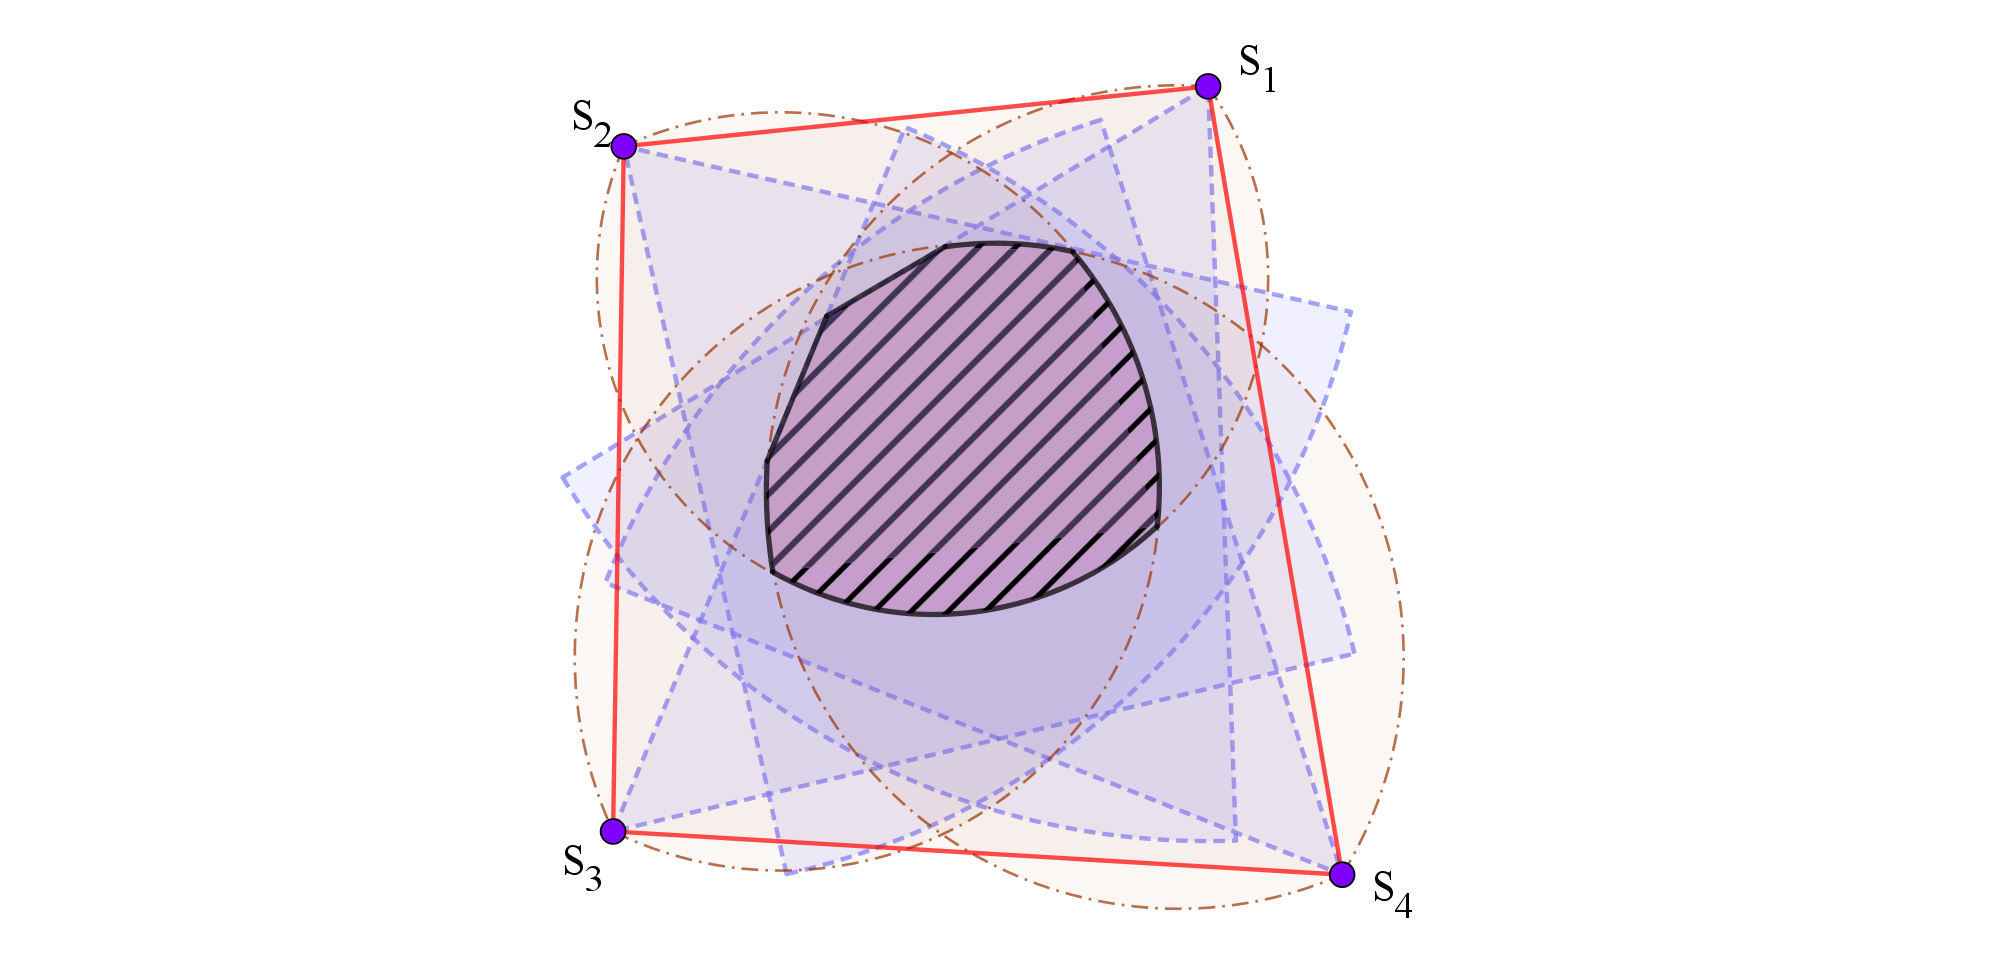
\includegraphics[scale=0.9]{hinhminhhoa.png}
\end{minipage}
\caption{($k-\omega$) region of $L=\{S_1,S_2,S_3,S_4\}$ and $\omega = 60$}
\end{figure}
